\documentclass[a0,final,landscape]{a0poster}
\usepackage{epsfig}
\usepackage{booktabs}
\usepackage{multicol}
\usepackage{pstricks,pst-grad}
\usepackage{url}
\usepackage{subfig}
\usepackage{float}
\usepackage{graphicx}
\usepackage{amsmath} 
\usepackage{amssymb}
\usepackage{tcolorbox}
\usepackage{booktabs}
\usepackage{multirow}
\usepackage{array}
\usepackage{tabulary}
\usepackage{caption}
\usepackage{tikz}
    \usetikzlibrary{shadows}
\usepackage{tcolorbox}
    \tcbuselibrary{skins}

\newcolumntype{K}[1]{>{\centering\arraybackslash}p{#1}}
\definecolor{blue}{RGB}{9,14,159}
\definecolor{vino}{RGB}{153,0,0}
\definecolor{cyan}{RGB}{24,116,205}
\definecolor{blue1}{RGB}{0, 0, 102}
\definecolor{green}{RGB}{0.61,0.73,0.35}
\newcommand\PaneW{390mm}
\setlength{\columnsep}{3cm}
\setlength{\columnseprule}{2mm}
\setlength{\parindent}{0.0cm}



\newcommand{\mytitle}[1]{
    \node[fill=vino, rounded corners, draw=white, line width=2pt, drop shadow, text width=12cm, inner sep=8pt, xshift=-2cm]
    at (frame.north){\bfseries\textcolor{white}{#1}};}

\newtcolorbox{mybox}[2][width=35cm]{enhanced, overlay={\mytitle{#2}}, borderline={2.5pt}{0mm}{vino}, borderline={.7pt}{1mm}{blue1},
    frame hidden, arc=3mm, sidebyside, lefthand width=30cm, segmentation hidden, top=15pt, #1 }


\newcommand{\pbox}[4]{
%\psshadowbox[#3]{
\begin{minipage}[t][#2][t]{#1}
#4
\end{minipage}
}

\newcommand{\background}[3]{
  \newrgbcolor{cgradbegin}{#1}
  \newrgbcolor{cgradend}{#2}
  \psframe[fillstyle=gradient,gradend=cgradend,
  gradbegin=cgradbegin,gradmidpoint=#3](0.,0.)(1.\textwidth,-1.\textheight)
}



\newenvironment{poster}{
  \begin{center}
  \begin{minipage}[c]{0.98\textwidth}
}{
  \end{minipage} 
  \end{center}
}



\newenvironment{pcolumn}[1]{
  \begin{minipage}{#1\textwidth}
  \begin{center}
}{
  \end{center}
  \end{minipage}
}


\newrgbcolor{lcolor}{0. 0. 0.80}
\newrgbcolor{gcolor1}{1. 1. 1.}
\newrgbcolor{gcolor2}{.80 .80 1.}



\setcounter{figure}{1}
\newcommand{\mycaption}[1]{
  \vspace{-0.4cm}
  \centering
  \begin{quote}
  \begin{center}
  {\footnotesize {\sc Figure} \arabic{figure}: #1}
  \end{center}
  \end{quote}
  \stepcounter{figure}
  
  
\def\@fnsymbol#1{\ensuremath{\ifcase#1\or *\or \dagger\or \ddagger\or
   \mathsection\or \mathparagraph\or \|\or **\or \dagger\dagger
   \or \ddagger\ddagger \else\@ctrerr\fi}}
  
}

\begin{document}

%\background{1. 1. 1.}{1. 1. 1.}{0.5}
\vspace*{2cm}
\newrgbcolor{lightblue}{0. 0. 0.80}
\newrgbcolor{white}{1. 1. 1.}
\newrgbcolor{whiteblue}{.80 .80 1.}


%%%%%%%%%%%%%%%%%%%%%%%%%%%%%%%%%%%%%%%%%%%%%
%%%      TITLE & AUTHORS
%%%%%%%%%%%%%%%%%%%%%%%%%%%%%%%%%%%%%%%%%%%%%
% Header
\vspace{-3.9cm}
\begin{poster}
\begin{center}
\begin{pcolumn}{0.99}
\begin{minipage}[c][8cm][c]{0.1\textwidth}
  \begin{center}
    \vspace{-0.5cm}
    \hspace{-1cm}
    
\includegraphics[scale=1.5]{img/UofC-vert.png}
  \end{center}
\end{minipage}
\begin{minipage}[c][10cm][c]{0.78\textwidth}
  \begin{center}
    {\veryHuge \textcolor{blue1}{\textbf{Title here using the largest font size of your entire poster to be eye catching. Keep it as short as possible}}}\\
    \Huge E. Barreto-Ojeda, Author 1, Author 2, Supervisor/Boss \\
    \LARGE Department of Biological Sciences and Centre for Molecular Simulation, University of Calgary.\\
    \LARGE estefania.barretooje@ucalgary.ca\hspace{2cm} supervisor@institution.ca
  \end{center}
\end{minipage}
\begin{minipage}[c][8cm][c]{0.08\textwidth}
  \begin{center}
    \hspace{1cm}
    
\includegraphics[scale=1.3]{img/cms_logo.jpg}
  \end{center}
\end{minipage}
\vspace{0.5cm}
\begin{center}
\hspace{-1cm}\noindent\textcolor{blue1}{\rule{110cm}{0.2pt}}
\end{center}
\end{pcolumn}
\end{center}
\end{poster}

%%%%%%%%%%%%%%%%%%%%%%%%%%%%%%%%%%%%%%%%%%%%%%%%%%%%%%%%%%%%%%%%%
%%% Introduction
%%%%%%%%%%%%%%%%%%%%%%%%%%%%%%%%%%%%%%%%%%%%%%%%%%%%%%%%%%%%%%%%%

\vspace{20cm}
%\hspace{-2.9cm}
\begin{minipage}[c][30cm][c]{0.32\textwidth}
\section*{\textcolor{blue1}{\Huge \bf{Introduction}}}
\vspace{-1cm}
\large
Academic posters are one of the best ways to showcase your research work at conferences and meetings. In contrast to oral presentations, audience in poster sessions are very dynamic. Hence, attractive designs and clear contents are key points to catch visitors. The best posters trigger discussions with the audience. So keep a clear plan of what to say when profs and senior students stand alongside your poster! In this template, I'll show you one of my preferred ways to include my research work in a LaTex poster. My research work is in computational biphysics. Hence, here I introduce the biomolecular system I working with (protein and its role, membranes,etc). I always highlight the medical relevance and specify if it is involved in therapeutics or treatments.\\

%%%%%%%%%%%%%%%%%%%%%%%%%%%%%%%%%%%%%%%%%%%%%%%%%%%%%%%%%%%%
%       METHODS
%%%%%%%%%%%%%%%%%%%%%%%%%%%%%%%%%%%%%%%%%%%%%%%%%%%%%%%%%%%%

\vspace{-1cm}
\section*{\textcolor{blue1}{\Huge \bf{Methods}}}
\vspace{-0.8cm}
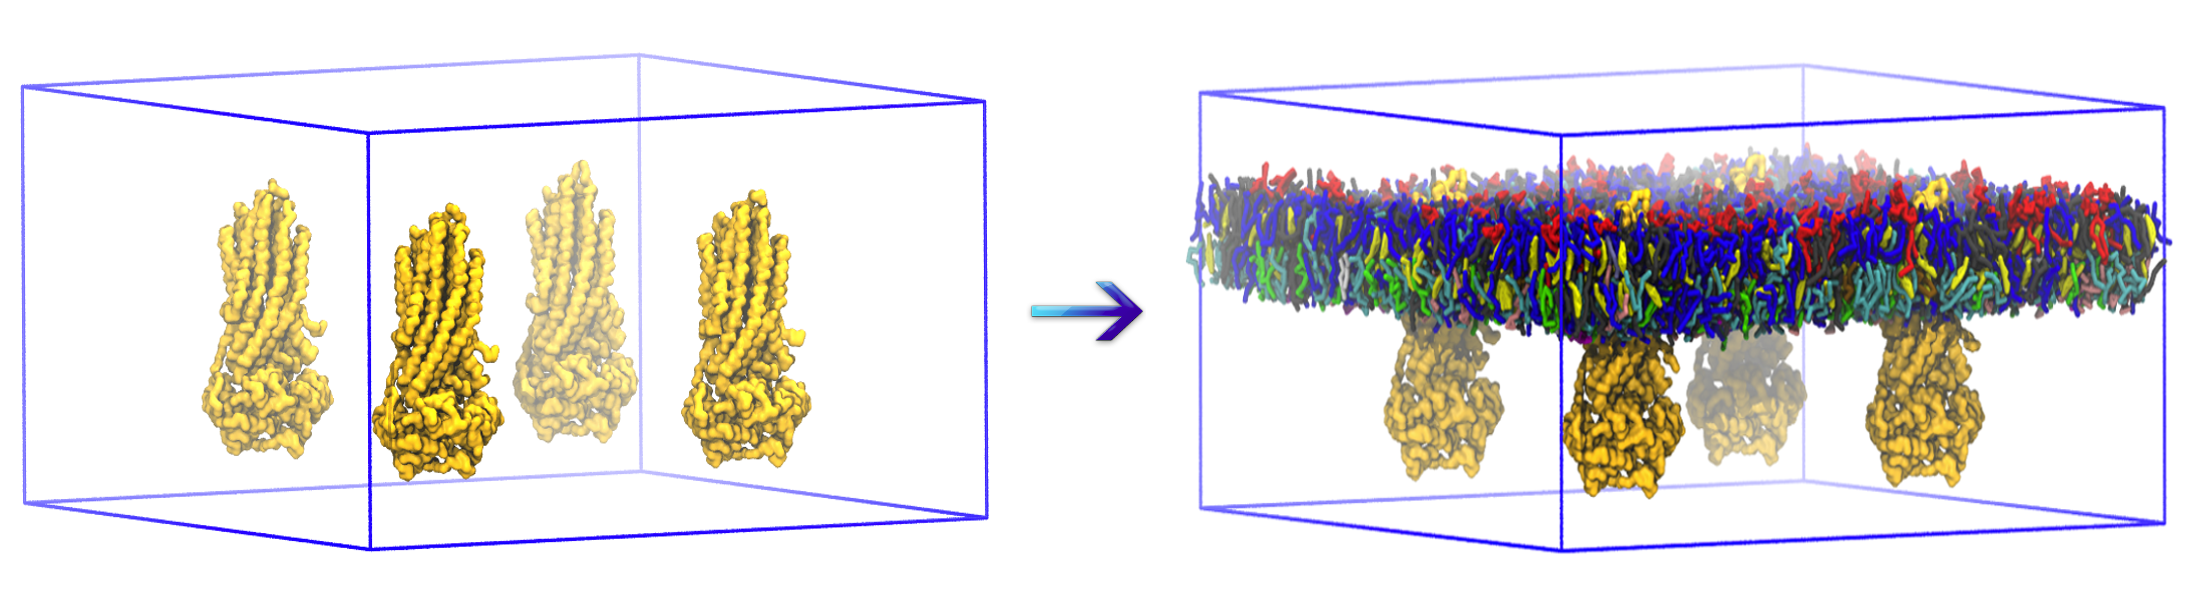
\includegraphics[scale=0.47]{img/system1.png} \\
\vspace{-1cm}
\begin{center}
\small{\textbf{Fig 1.} Simulation box system set up. Box Size: 40x40x18 nm.\\}
\end{center}

\begin{center}
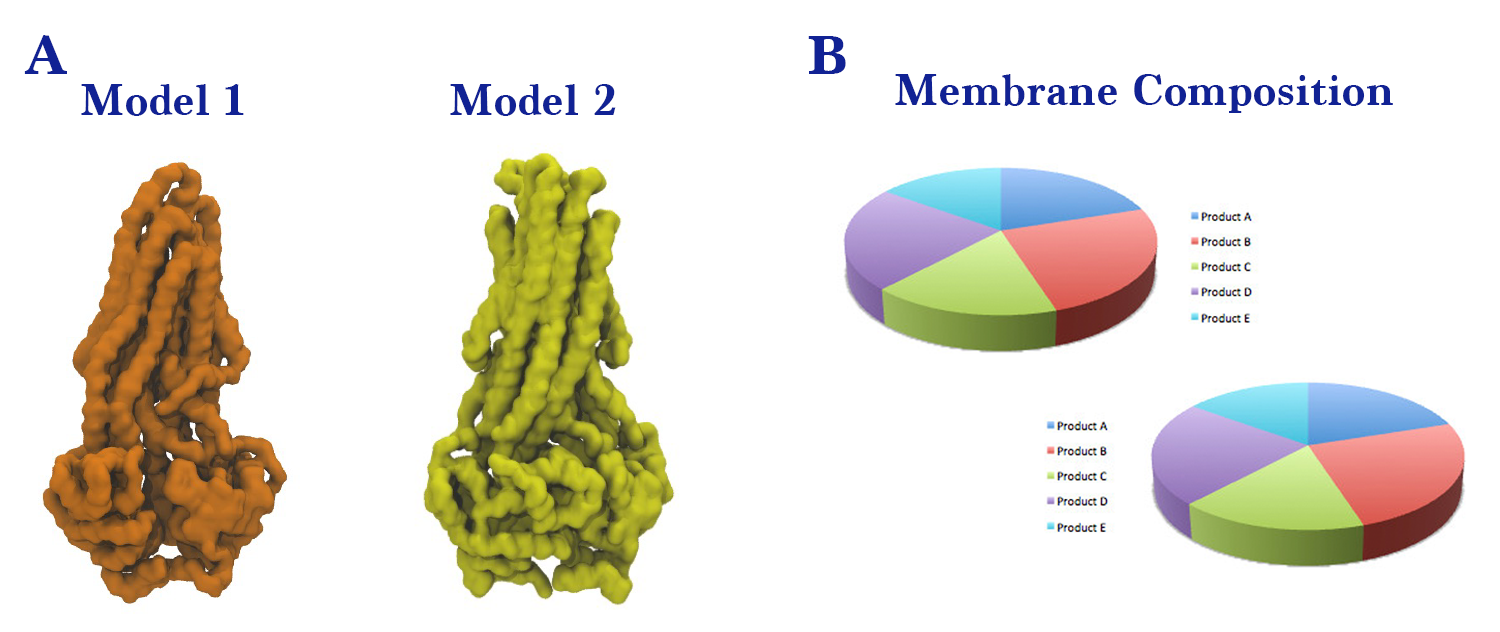
\includegraphics[scale=2.5]{img/pies-1.png}\\
\vspace{-0.2cm}
\small{\textbf{Fig 2.} A) Protein model 1 and 2, for the open and closed state, respectively. B) Lipid bilayer composition by lipid head groups.}
\end{center}
\large
The methods section includes basic parameters/protocols, duration of the study when relevant , inclusion/exclusion criteria, statistical analysis, key approaches and primary features of the data $[1]$. For example, since I work on MD, I use to describe my simulation box(es). Each system contains four molecules of the same protein. My system usually have $\sim$ 6000 molecules. Simulations were carried out for 20$\mu$s. Analysis were carried out using different GROMACS tools, and in house software.


%%%%%%%%%%%%%%%%%%%%%%%%%%%%%%%%%%%%%%%%%%%%%%%%%%%%%%%%%%%%
%   Conclusions
%%%%%%%%%%%%%%%%%%%%%%%%%%%%%%%%%%%%%%%%%%%%%%%%%%%%%%%%%%%%
\vspace{-0.5cm}
\section*{\textcolor{blue1}{\Huge \bf{Concluding Remarks}}} 
\vspace{-0.8cm}
\large
Conclusions must derive from the results section (here on the middle and right columns). For example, MD simulations were performed to investigate a specific feature of a given protein. After 20$\mu$s of simulation time, we observed a characteristic/relevant dynamic in lipids that persists in the models. During our 20$\mu$s-long simulations, the number of lipids (LIPID1) around the protein increases/decreases, while the number of cholesterol increases meaningfully. This result matches with the experimental results reported by Reference1, Reference2. This analyses suggest something about the lipids or the protein of interest. We could explain why (i.e. electrostatic interactions, electric potential, etc). Offer a sensible explanation of your findings. Finally, a last sentence that encloses the relevance or importance of performing this study and the results obtained.  

\end{minipage}




%%%%%%%%%%%%%%%%%%%%%%%%%%%%%%%%%%%%%%%%%%%%%%%%%%%%%%%%%%%%%%%%%%%%%5


\vspace{-15.2cm}
\hspace{39cm}
\begin{minipage}[c][-30cm]{0.3\textwidth}
\section*{\textcolor{blue1}{\Huge \bf{Results}}} 
\vspace{-0.5cm}
\Large\textcolor{vino}{\textbf{Model 1}}\\
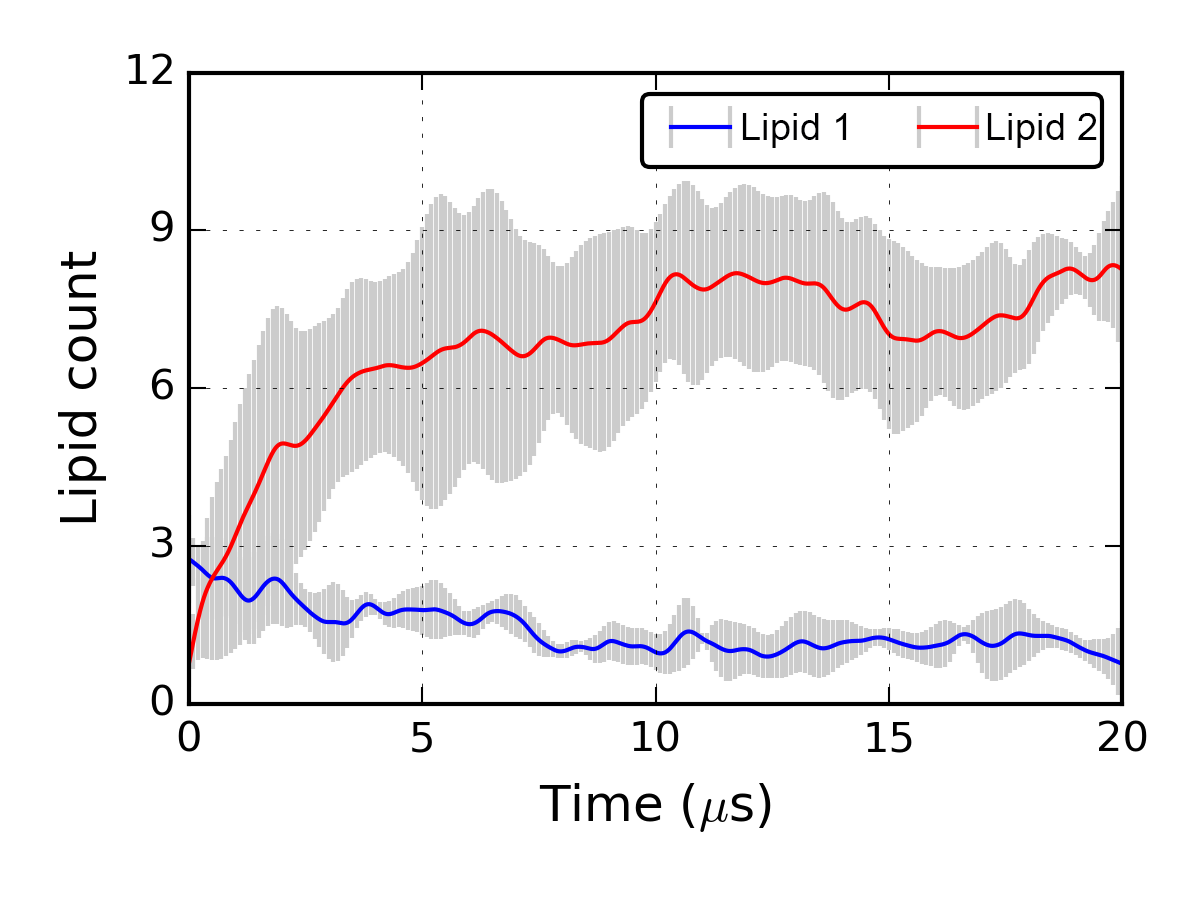
\includegraphics[scale=1.7]{img/Model1_Lipid12.png}
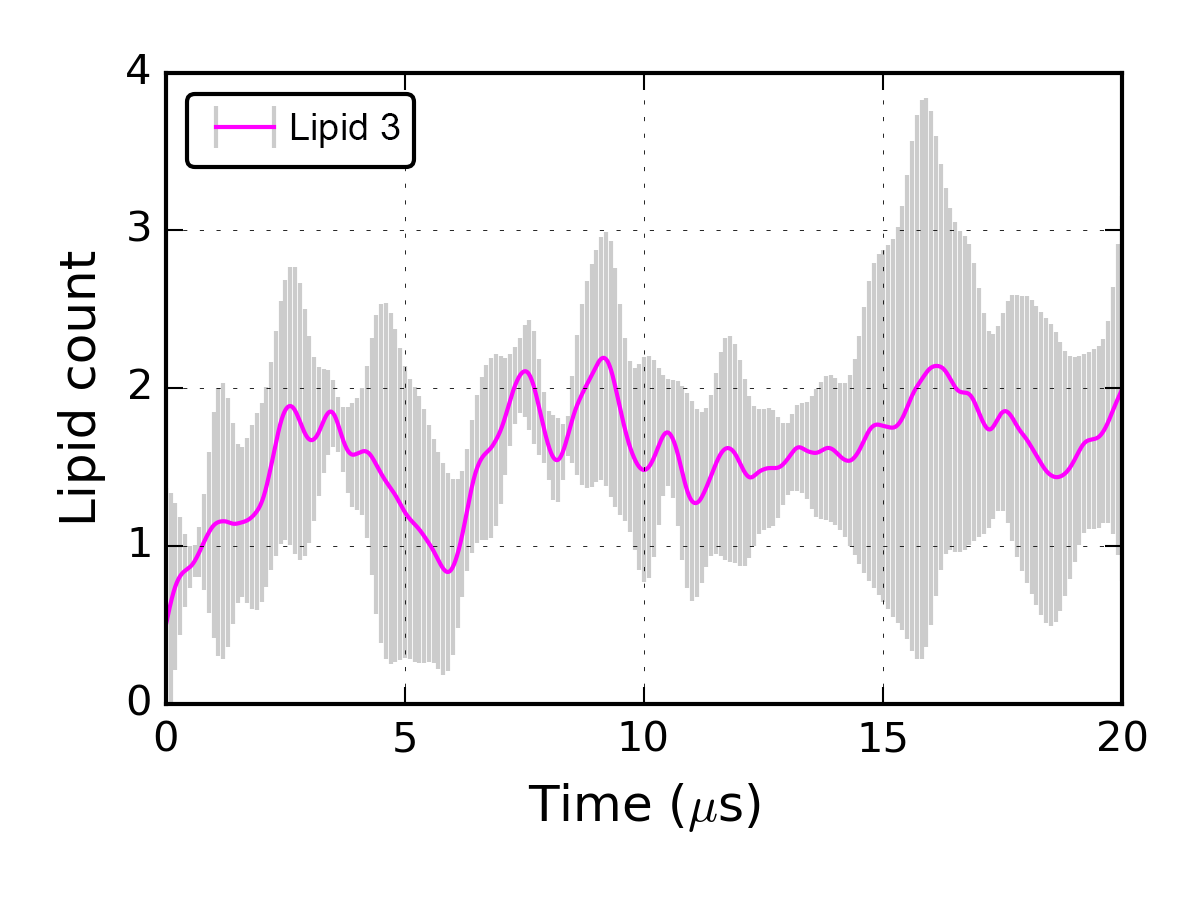
\includegraphics[scale=1.7]{img/Model2_Lipid3.png}\\ 
\Large\textcolor{vino}{\textbf{Model 2}}\\
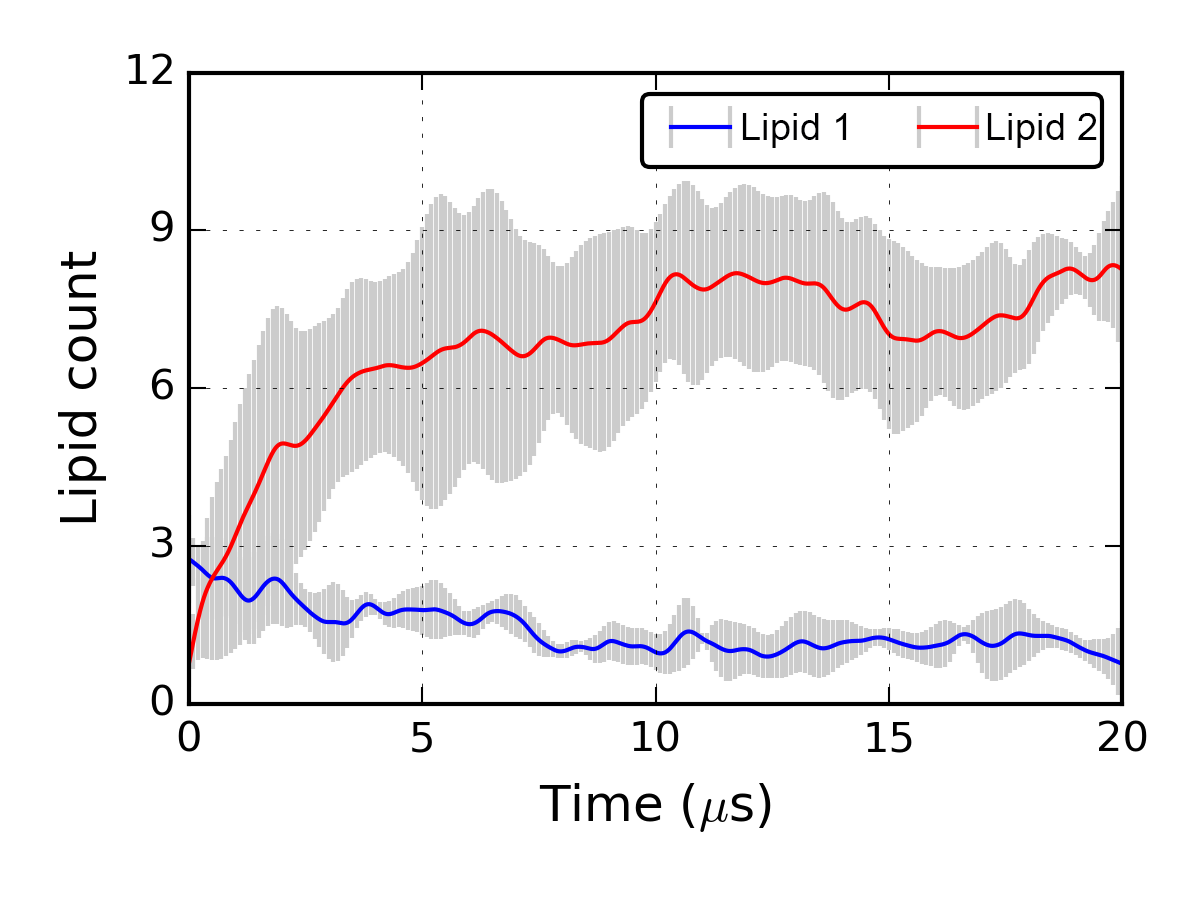
\includegraphics[scale=1.7]{img/Model1_Lipid12.png}
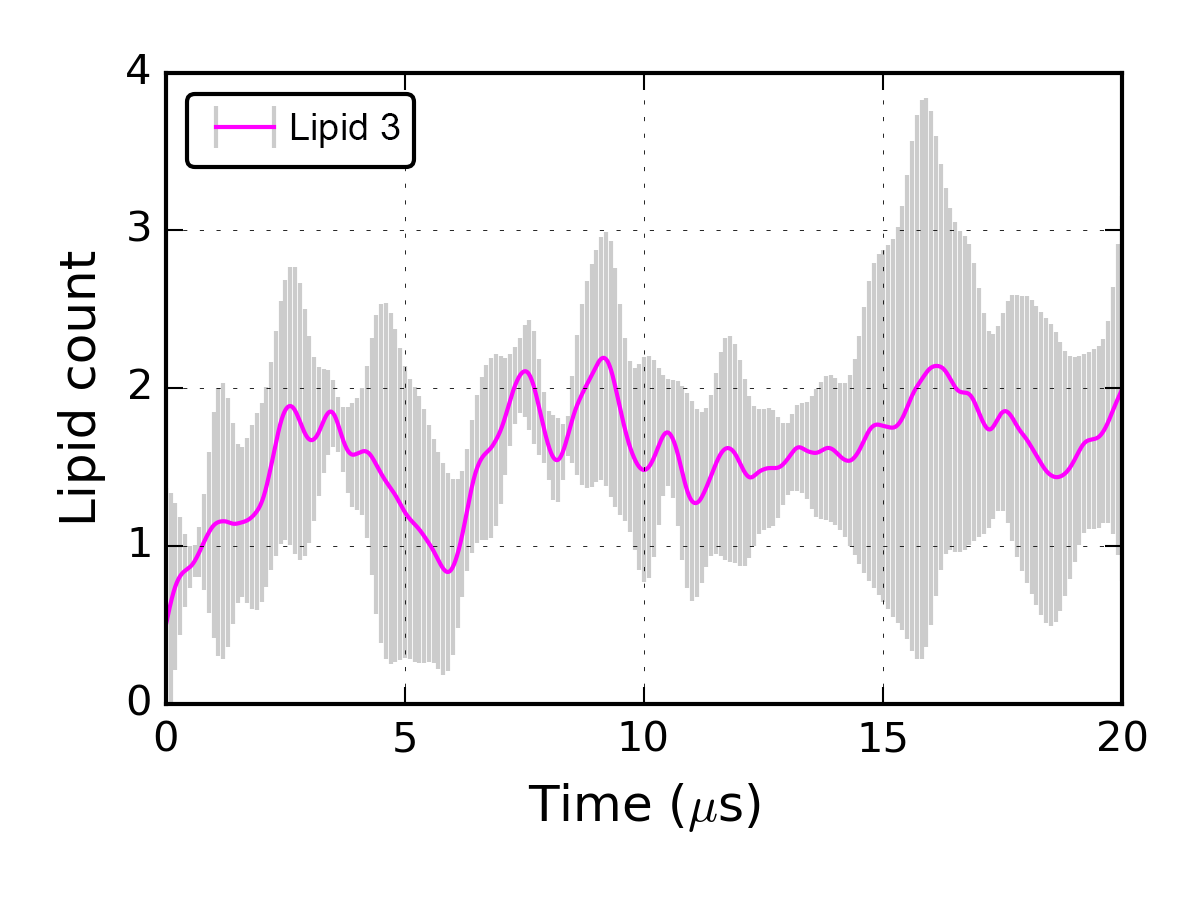
\includegraphics[scale=1.7]{img/Model2_Lipid3.png}\\
\begin{center}
\small{\vspace{-1.5cm}\textbf{Figure 3.} Caption Figure 3. Give relevant details of the plots. Trends, convergence, similarities/differences.}
\end{center}
\vspace{0.5cm}
\hspace{1cm}
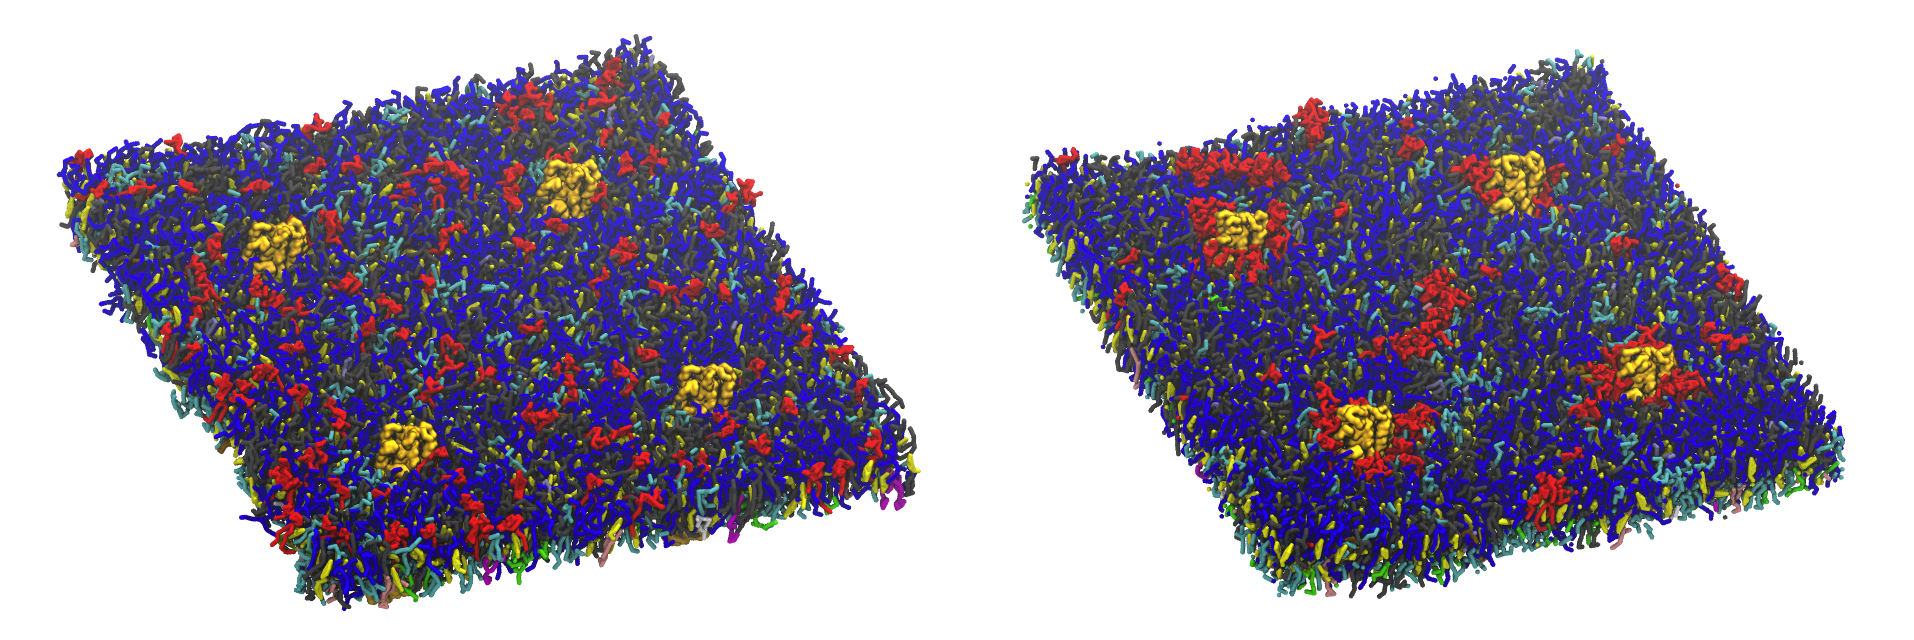
\includegraphics[scale=0.51]{img/snaps_white.png}\\
\vspace{-1cm}
\begin{center}
\hspace{2cm}\small{\textbf{Fig 4.} Use snapshots of your simulation from different views. I tend to add top views comparing two different simulation times. Here $t=1\mu$s (left) and $t=20\mu$s (right) for model 2.}
\end{center}
%\vspace{-1cm}
\LARGE \textbf{Feature X}\\
\vspace{-2cm}
\begin{center}
\hspace{1cm}\Large\textcolor{vino}{\textbf{Model 1}}\hspace{8cm}\textcolor{vino}{\textbf{Model 2}}\\
\hspace{2cm}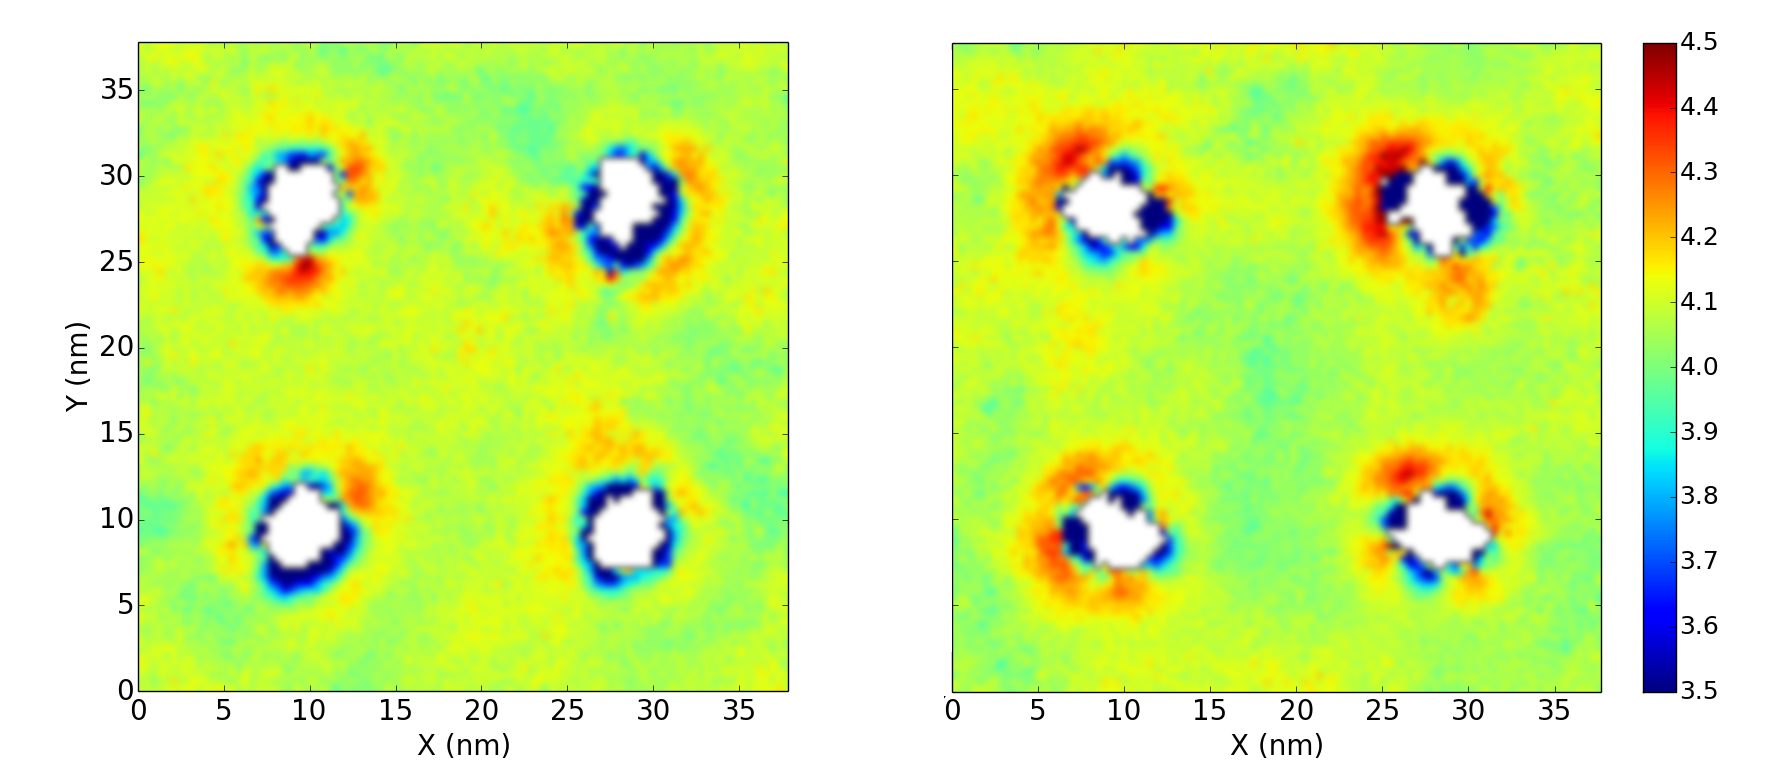
\includegraphics[scale=0.62]{img/thicks.png}\\ \hspace{2cm}
\small{\textbf{Fig 5.} 2D maps of some property, averaged over the last n nanoseconds. Use a decent colormap! The jet colormap included here is always my last option. Please, avoid it!}
\end{center}
\end{minipage}




\hspace{77cm}
\begin{minipage}[c][-30cm]{0.3\textwidth}
\LARGE \textbf{Feature Y}\\
%Lipid0
\Large\hspace{2cm}\textcolor{vino}{\textbf{Model 1}}\hspace{14 cm}\textcolor{vino}{\textbf{Model 2}}\\
\vspace{0.4cm} 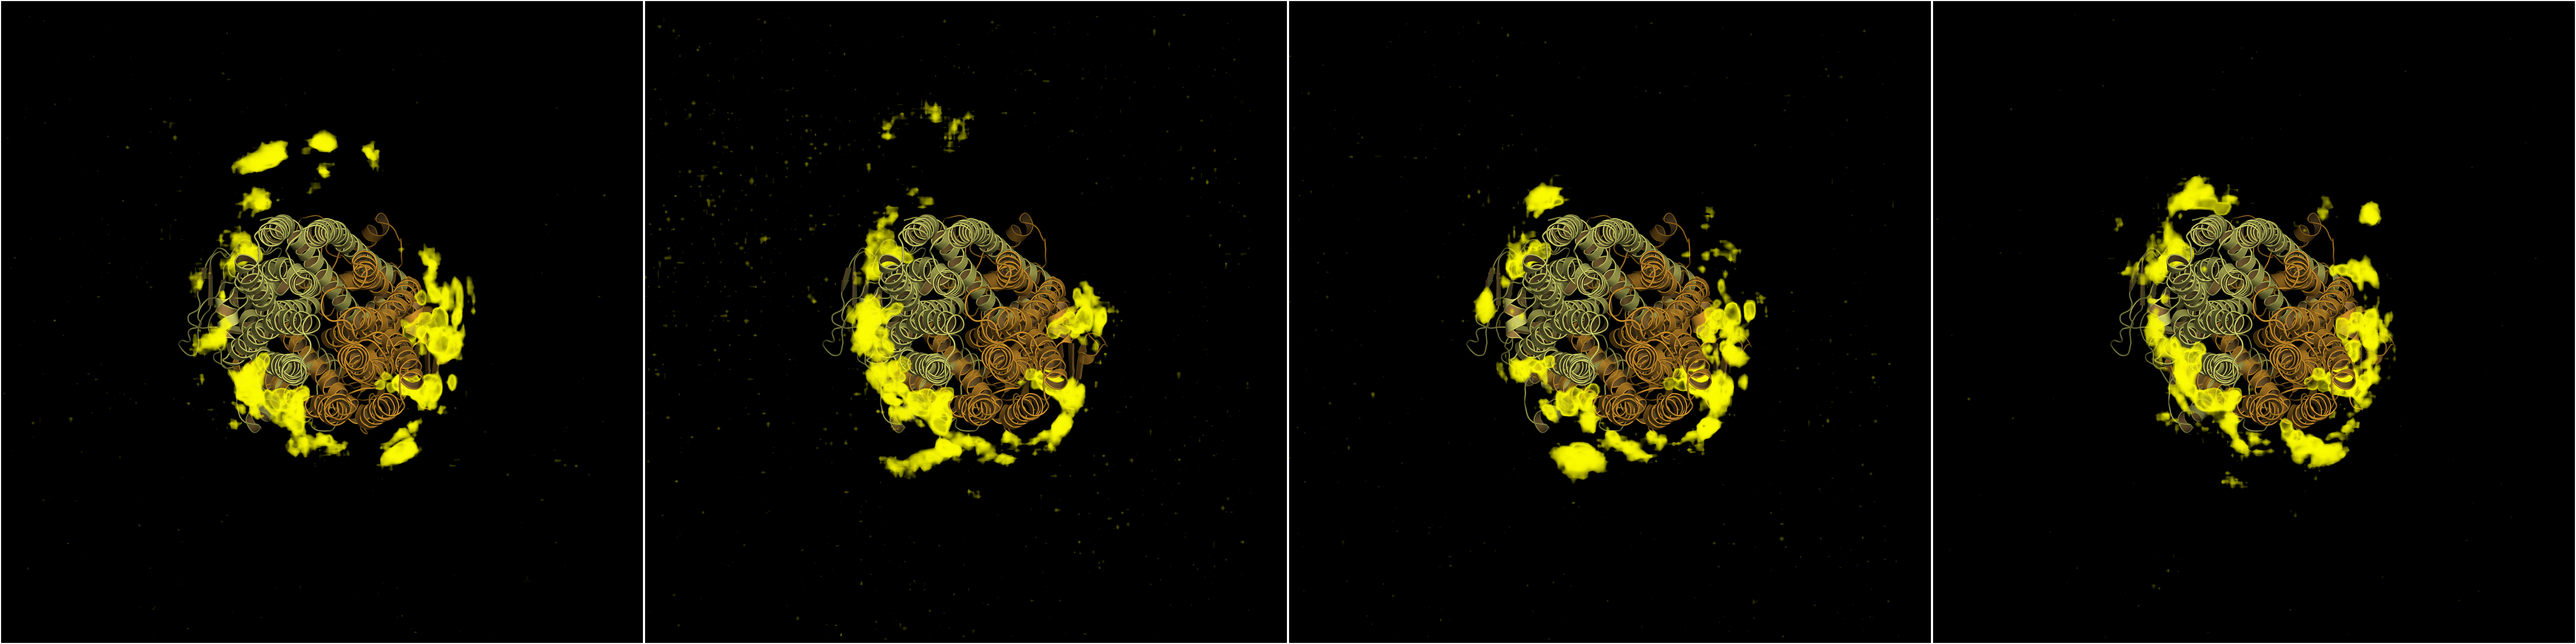
\includegraphics[scale=0.05]{img/Lipid0_M1.png} \hspace{1cm}
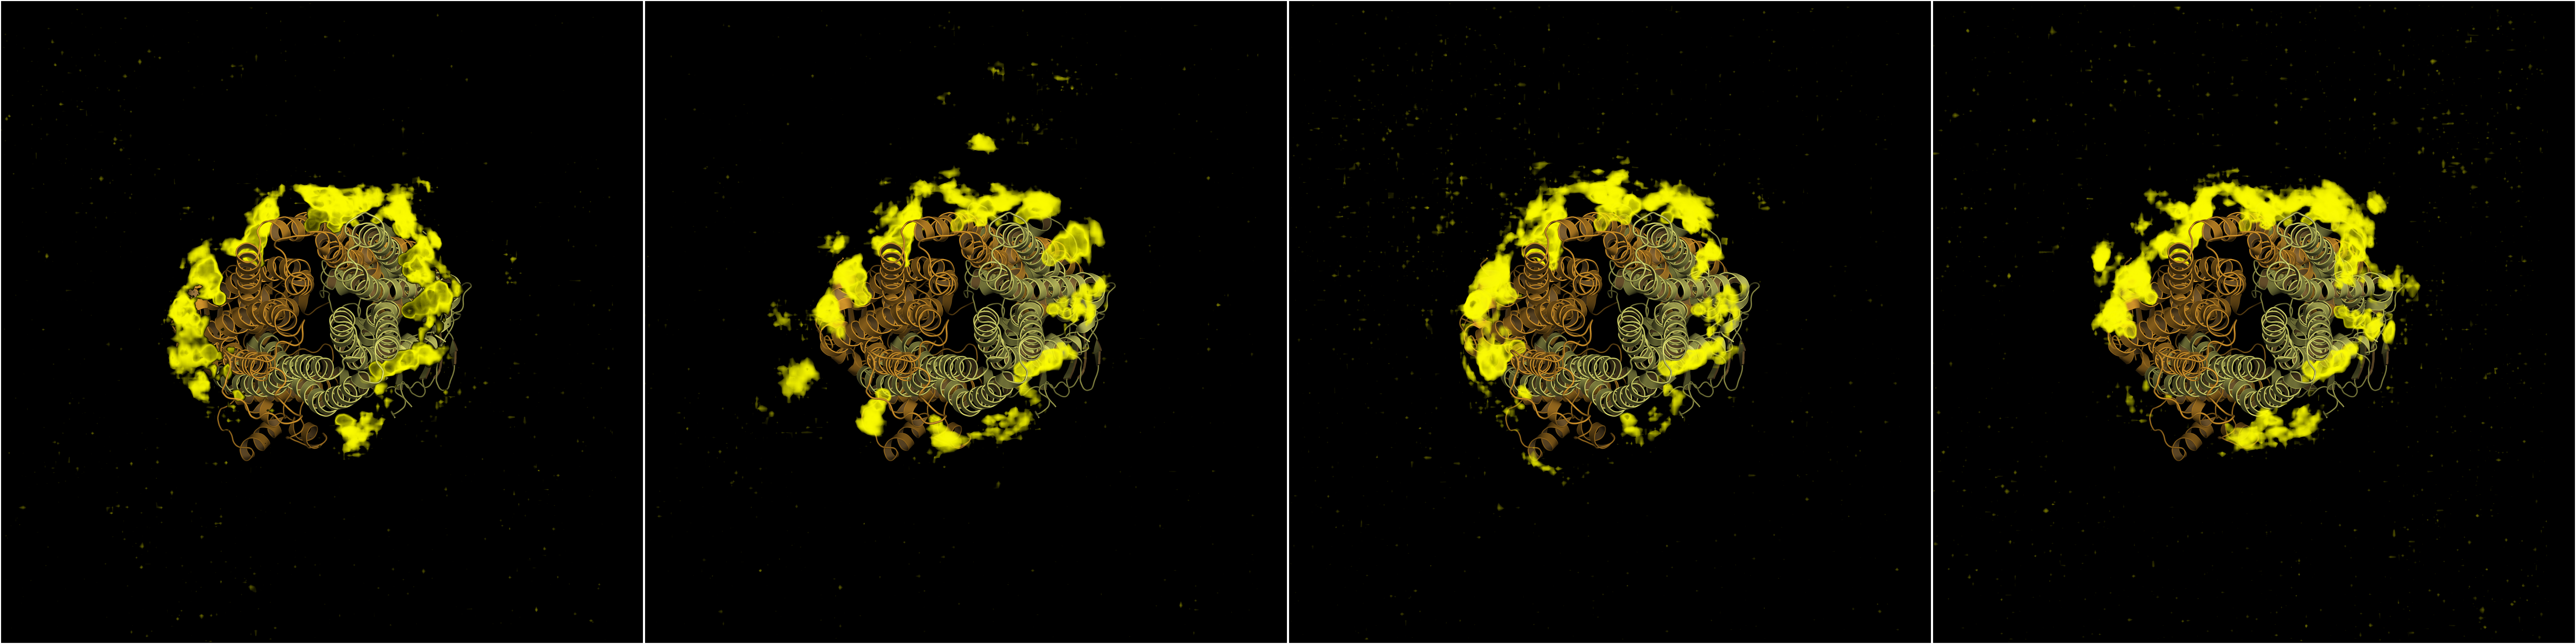
\includegraphics[scale=0.05]{img/Lipid0_M2.png} \\ \vspace{0.1cm} 
%Lipid1
\vspace{0.4cm} \includegraphics[scale=0.05]{img/Lipid1_M1.png}  \hspace{1cm} 
\includegraphics[scale=0.05]{img/Lipid1_M2.png}  \\ \vspace{0.1cm} 
%Lipid2
\vspace{0.4cm} 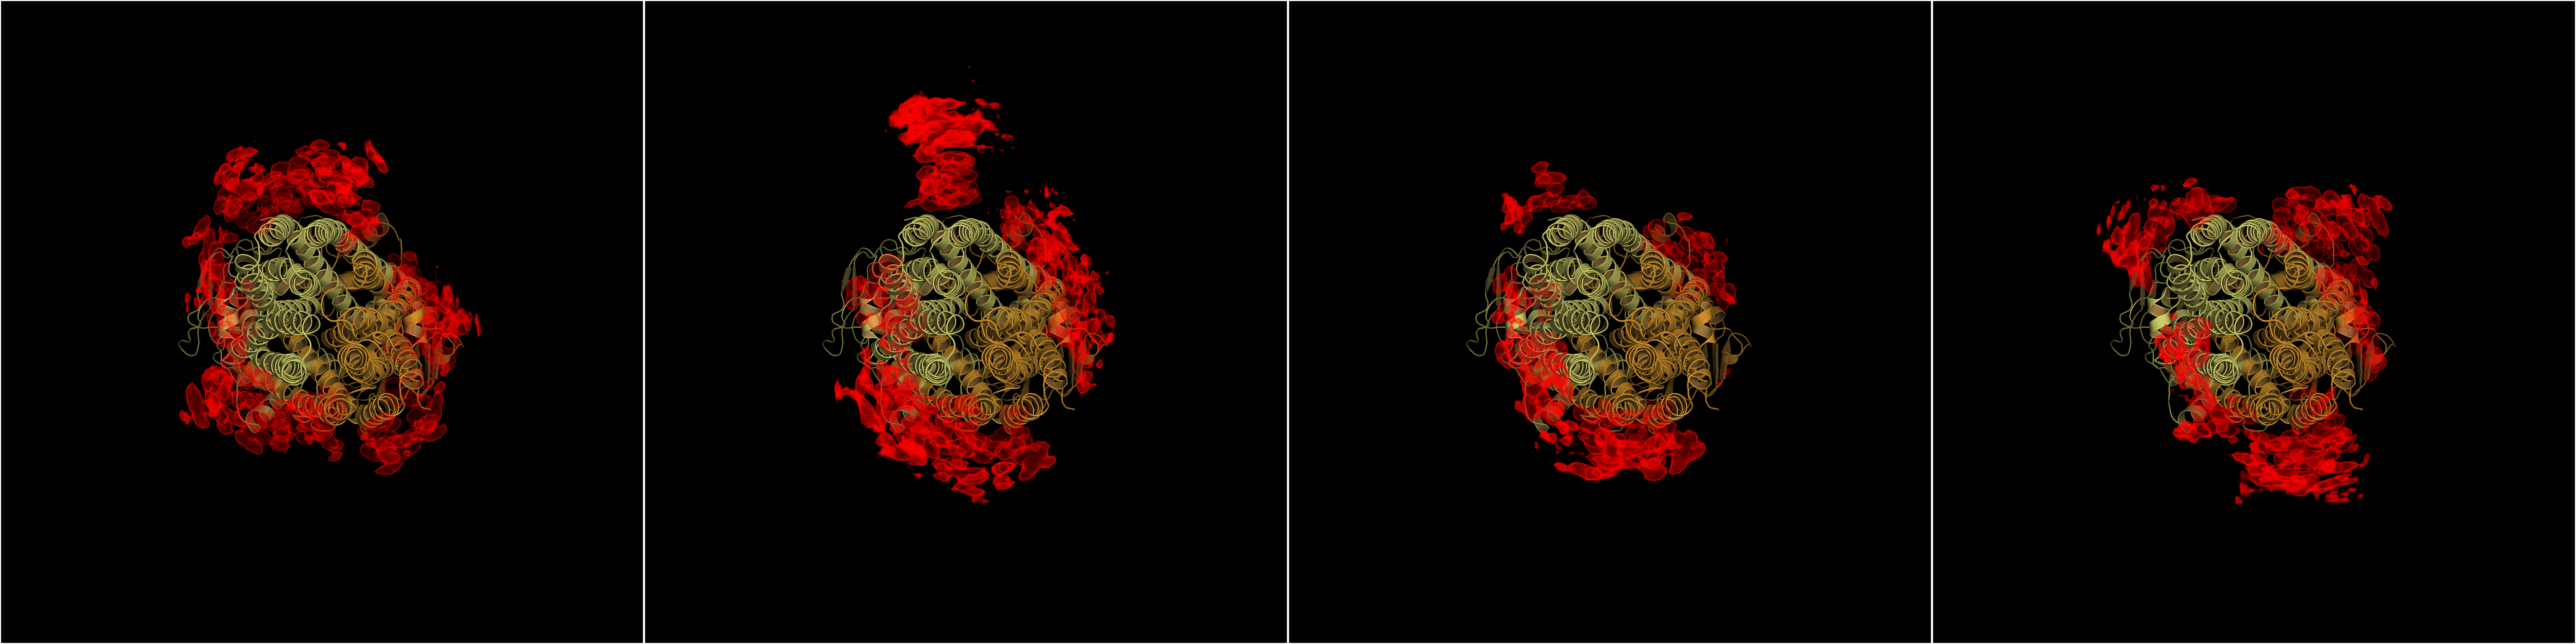
\includegraphics[scale=0.05]{img/Lipid2_M1.png}  \hspace{1cm} 
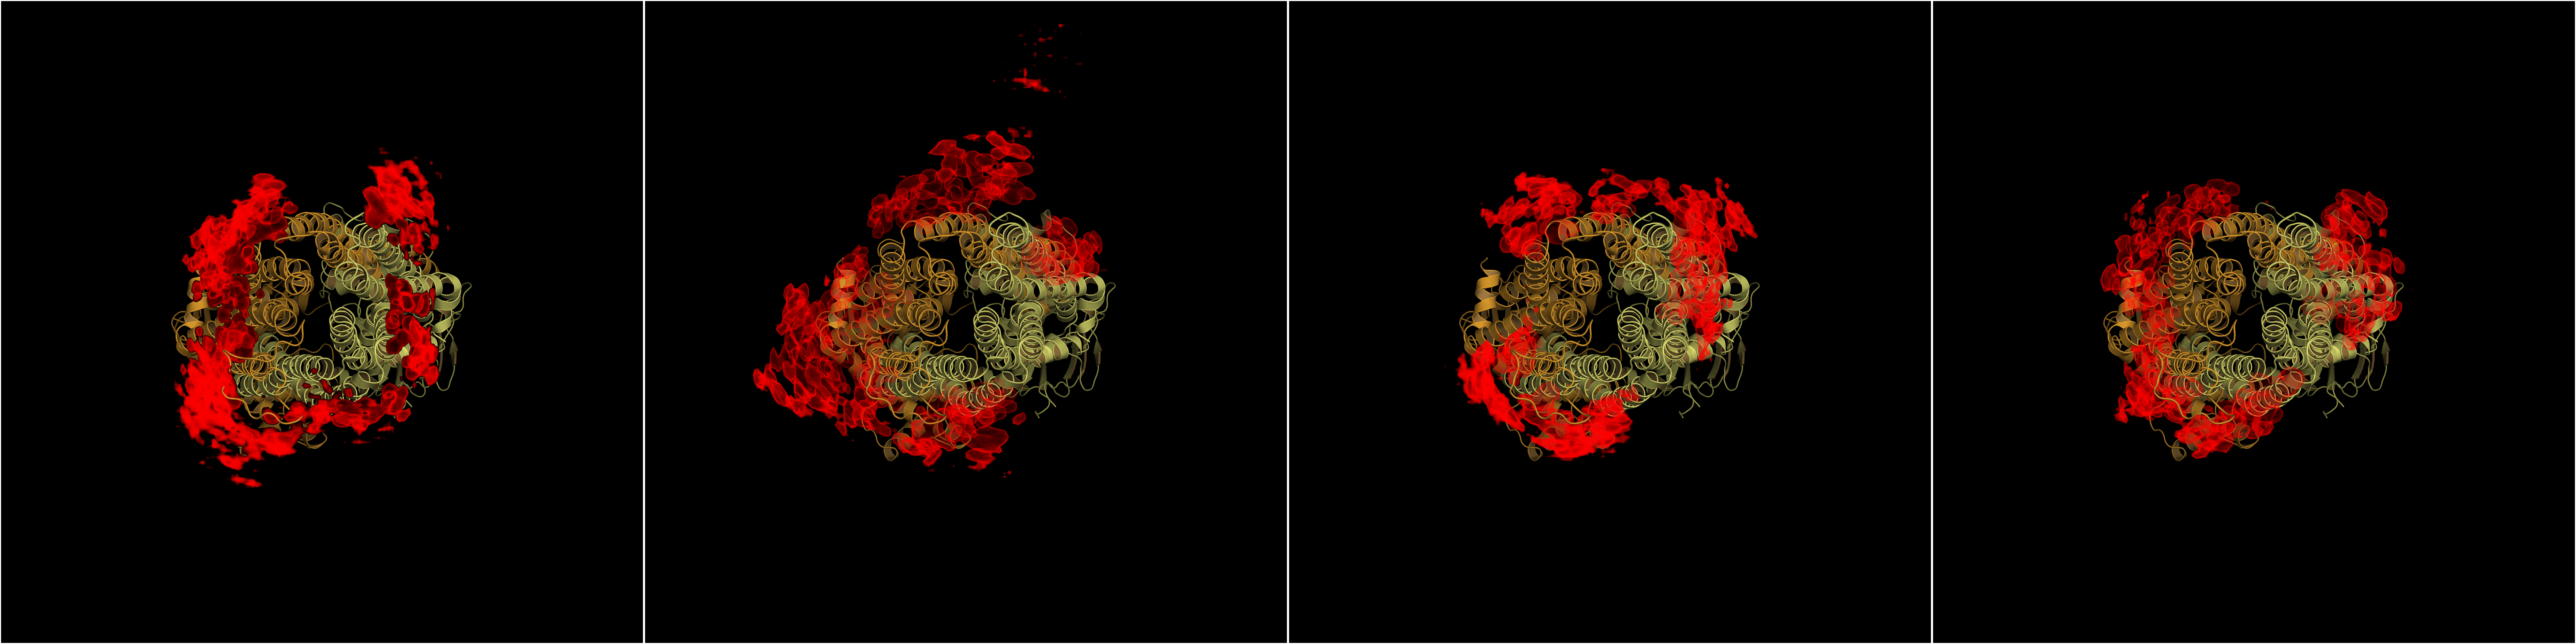
\includegraphics[scale=0.05]{img/Lipid2_M2.png}  \\ \vspace{0.1cm}
%Lipid3
\vspace{0.4cm} 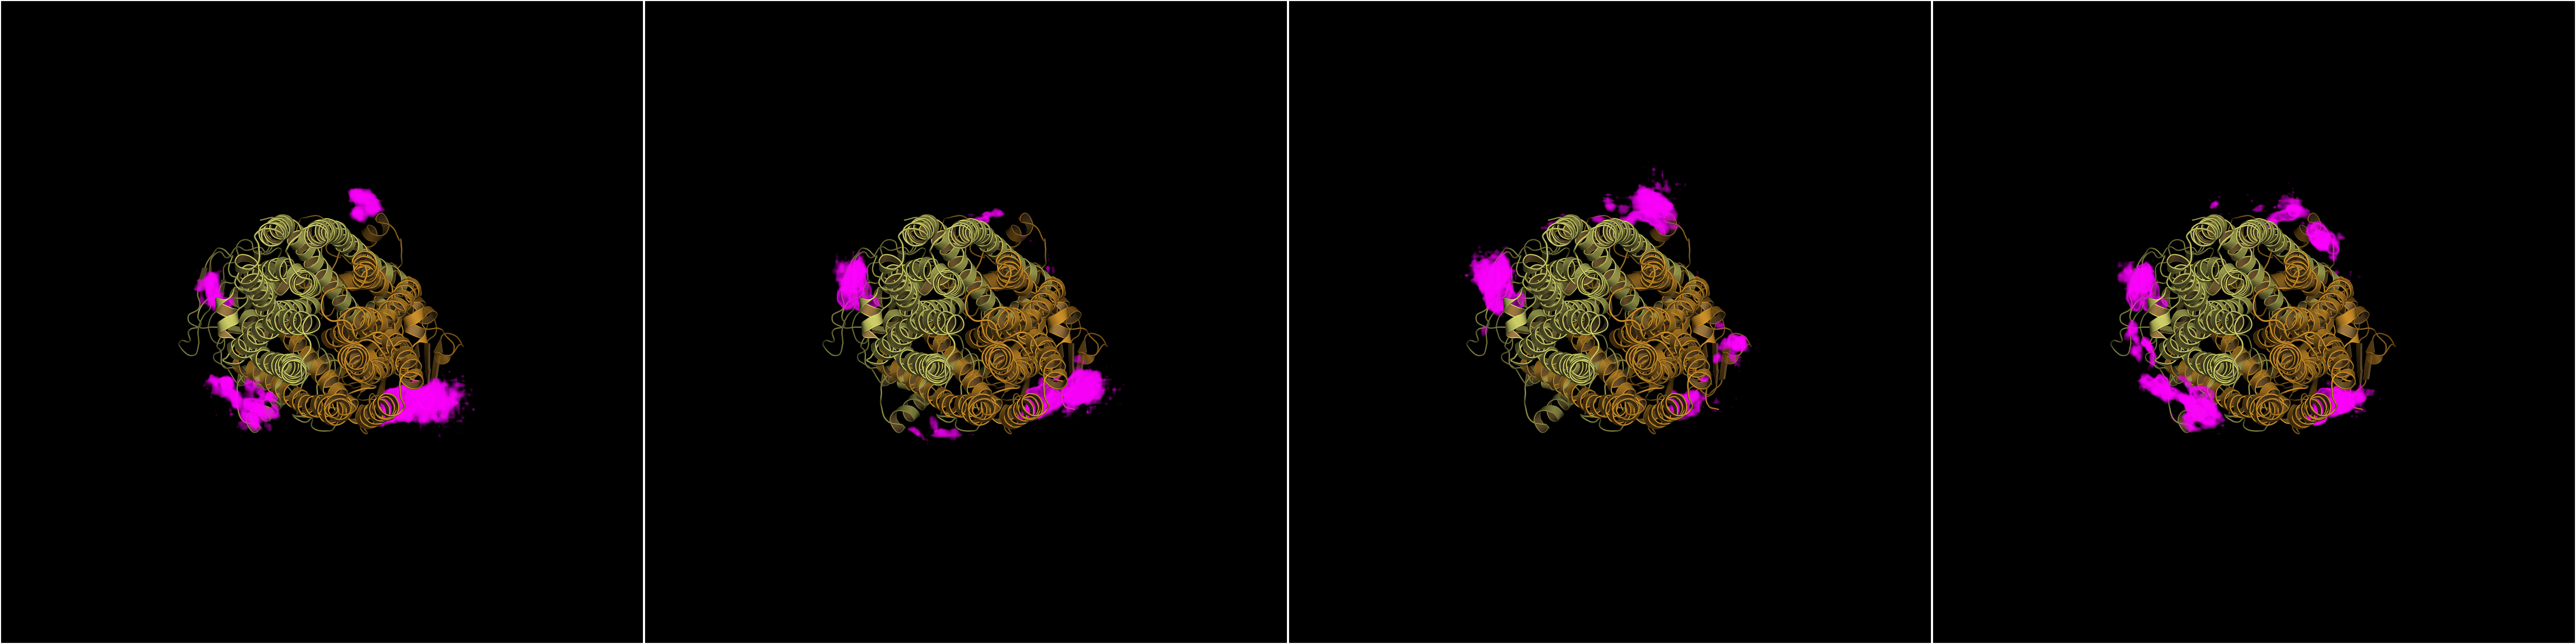
\includegraphics[scale=0.05]{img/Lipid3_M1.png}  \hspace{1cm} 
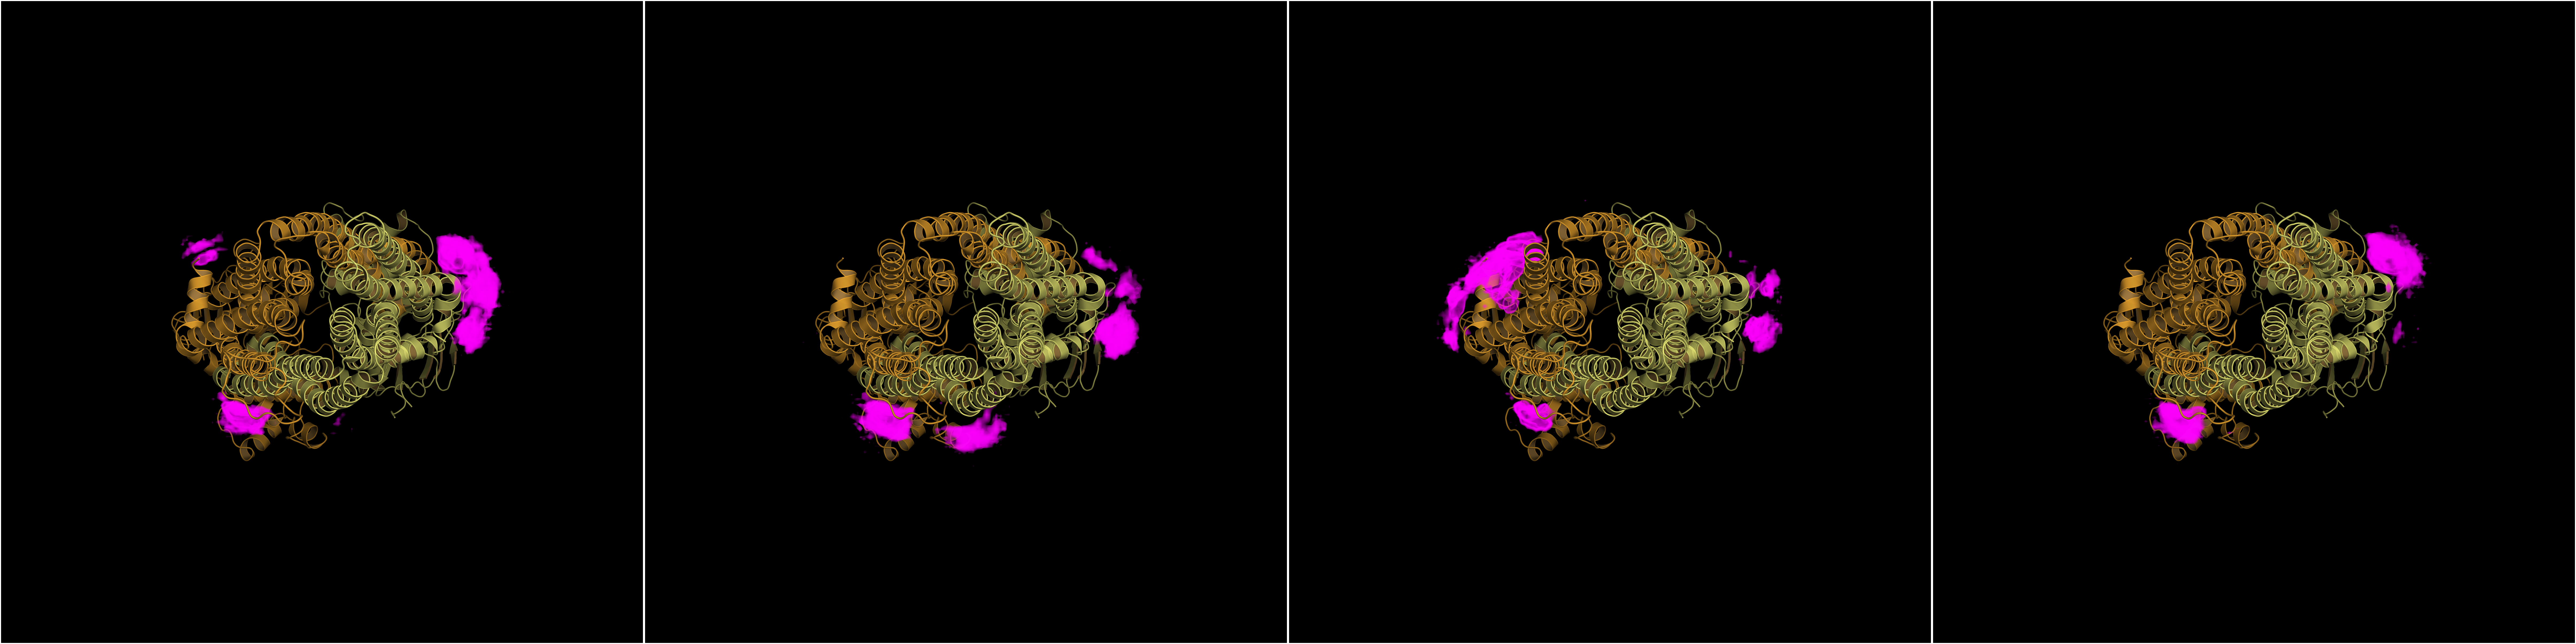
\includegraphics[scale=0.05]{img/Lipid3_M2.png}  \\ \vspace{0.1cm}
%Lipid 4
\vspace{0.4cm} \includegraphics[scale=0.05]{img/Lipid4_M1.png} \hspace{1cm}
\includegraphics[scale=0.05]{img/Lipid4_M2.png}
\begin{center}
\small{\textbf{Fig 6.} Add fancy plots. Usually 3D plots are more eye-catching than 2D plots. Specify what color means what. Here, lipid densities of LIPID0 (yellow), LIPID1 (red), LIPID2 (blue), and LIPID3 (magenta) lipids are shown. Densities were calculated over the last 2 $\mu$s of the simulation.}
\end{center}

\LARGE \textbf{Some Equations} \\
\vspace{-1cm}
\large
\begin{equation*}
\text{Equation X}=\frac{\text{A*x+C*y}_{n}}{\text{some text} \Sigma_{n=1}^{j}} 
\end{equation*}
\vspace{-1cm}
\begin{align*}
\text{Equation Y}=&\frac{\text{A*x+C*y}_{n}}{\text{some text} \Sigma_{n=1}^{j}} & \text{Ratio of Z}=&\frac{\text{A*x+C*y}_{n}}{\text{some text} \Sigma_{n=1}^{j}} &
\end{align*}
\vspace{-1cm}

\hspace{-2cm}
\Large\hspace{2cm}\textcolor{vino}{\textbf{Table Model 2}}
\begin{center}
\begin{tabular}{K{5.5cm}K{6cm}K{8cm}K{6cm}K{8cm}}
        &              & Value (units) &              &                           \\ \cline{2-4}
        & $n=1$          & $n=2$         & $n=3$          &                           \\ \cline{1-4}
CHOL    & 0.5$\pm$0.1  & 0.9$\pm$0.1 & 0.9$\pm$0.1  & \small{Feature 1}       \\
LIPID1      & 0.5$\pm$0.1  & 2.4$\pm$0.1 & 2.0$\pm$0.4  & \small{Feature 2}  \\
LIPID2      & 0.5$\pm$0.1  & 1.2$\pm$0.2 & 1.2$\pm$0.2  & \small{Feature 3}   \\
Others  & 0.5$\pm$0.1  & 1.0$\pm$0.1 & 1.0$\pm$0.1  & \small{No feature} \\ \cline{1-4} \\
\end{tabular}
\end{center}
\vspace{-1cm}
\Large\textcolor{vino}{\textbf{Table Model 2}}
\vspace{-1cm}
\large
\begin{center}
\begin{tabular}{K{5.5cm}K{6cm}K{8cm}K{6cm}K{8cm}}
        &              & Value (units) &              &                           \\ \cline{2-4}
        & $n=1$          & $n=2$         & $n=3$          &                           \\ \cline{1-4}
CHOL    & 0.4$\pm$0.1  & 0.9$\pm$0.1 & 0.9$\pm$0.1  & \small{Feature 1}       \\
LIPID1      & 0.4$\pm$0.1  & 2.4$\pm$0.1 & 2.0$\pm$0.4  & \small{Feature 2}  \\
LIPID2      & 0.4$\pm$0.1  & 1.2$\pm$0.2 & 1.2$\pm$0.2  & \small{Feature 3}   \\
Others  & 0.4$\pm$0.1  & 1.0$\pm$0.1 & 1.0$\pm$0.1  & \small{No feature} \\ \cline{1-4} \\
\end{tabular}
\end{center}
%\vspace{-1cm}
%\small{PU: Poly-unsaturated. FS: Fully saturated. Others: Neither fully saturated nor poly-saturated.\\}
%\end{center}
\vspace{-2.5cm}
\section*{\textcolor{blue1}{\Large \bf{References}}}
\vspace{-1cm}
\tiny{
\begin{enumerate}
 \item Gundogan B, Koshy K, Kurar L, Whitehurst K. How to make an academic poster. \textit{Ann Med Surg (Lond)}. 2016;11:69-71. Published 2016 Sep 6. 
 \item Authors. Title. Journal. Year. Issue. pages-pages.
\end{enumerate}
}
\vspace{-1.2cm}
%\begin{mybox}{Acknowledgments}
\section*{\textcolor{blue1}{\Large \bf{Acknowledgments}}}
\begin{center}
\vspace{-0.5cm}

\includegraphics[scale=0.7]{img/CCanada_logo.png}

\includegraphics[scale=0.18]{img/westgrid_logo.jpg}

\includegraphics[scale=0.7]{img/AB_logo.jpg}
\end{center}
%\end{mybox}

\end{minipage}


\end{document}





